\documentclass[../main.tex]{subfiles}
\begin{document}
\chapter{背景}

\section{水球の関連知識}
\textgt{水球}
\par 水球とは,縦30m横25mのプールを使用して行われる球技である.各チーム,ゴールキーパー1名を除き6名のフィールドプレーヤーがおり,
ゴールキーパー以外は片手でのみボールを扱うことができる.8分×4ピリオドの試合時間の中で,より多くのゴールを決めたチームの勝ちとなる.

\textgt{パーソナルファウル}
\par 水球にはディフェンスの選手が犯すファウルとしてオーディナリーファウルとパーソナルファウルという2種類のファウルが存在している.
オーディナリーファウルの対象となるプレーは,ボールを持った相手を身体の正面から向かって沈めようとする行為などであり,
ボールを持っていた選手からのフリースローでプレーは再開される.これに対しパーソナルファウルの対象となるプレーは,
ディフェンスの選手がボールを持っていないオフェンスの選手を掴みその動きを阻害することや,オフェンス選手の身体に対して
背中側から沈めようとする行為などが対象となるファウルである.パーソナルファウルになった場合,状況によって審判は退水か5mペナルティーシュートの
判断を下す.退水となった場合,ファウルを犯した選手は20秒間フィールド外に設けられた退水ゾーンというエリアに入らなくてはならない.
これに対して5mペナルティーシュートではシューターはゴールから5m離れた位置から,ゴールキーパーと1対1でシュートを打つことになる.
このパーソナルファウルは2019年のルール改正以来増加しており,関東大学水球1部リーグの試合では2021年度には1試合平均12回だったが
2022年度には平均14回となっており,わずかながら回数の上昇が見られる.

\textgt{退水セット}
\par 上記の退水が発生した際,一時的にオフェンスが数的有利になる現象が起こる.この際のオフェンスを退水セットと呼び,
オフェンスを行っているチームにとって得点を取ることに有利な状況である.この機会を有効に活用するために各チーム戦術を練ることが多く,
本研究での実験対象とした.また退水セットでオフェンスがとる一般的な形として、ゴール付近の2mラインに
4名,ゴールから少し離れた6mライン付近に2名を配置する4-2システムが採用されている.このシステムでは次の図のように各ポジションに番号が
割り振られており,本研究内でもそのポジション番号を用いている.\ref{img:ExclusionNO}

\begin{figure}[ht]
    \begin{center}
        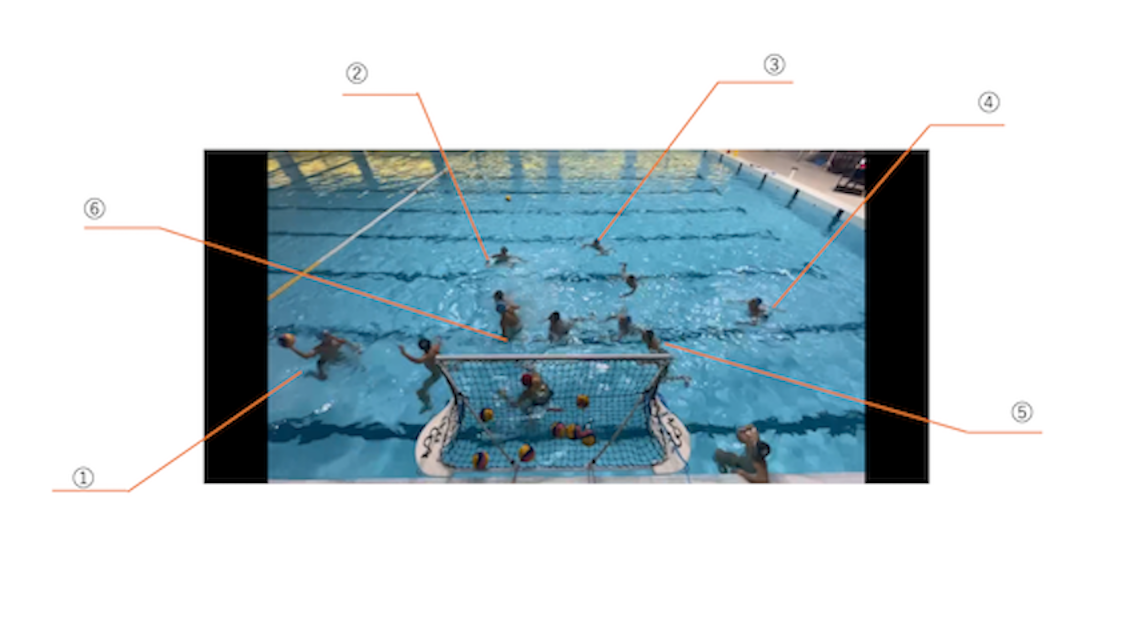
\includegraphics{img/01.png}
        \caption{退水セットでの4-2システムとポジション番号}
        \label{img:ExclusionNO}
    \end{center}
\end{figure}



\subsection{Tkinter}
\par TkinterはPythonの標準ライブラリの一つで,GUIアプリケーションを作成するためのフレームワーク.Tkinterを使用して,ウィンドウ・ボタン・ラベルなどのグラフィカルユーザインタフェース部品を簡単に作成することができる.

\section{先行研究}
\subsection{退水セットの攻め方}
\par 水球の退水セットにおける分析は多数存在している.日本国内の高校総体から東京オリンピックまでの退水セットの攻め方を分析した研究\cite{weko_1697_1}
では,欧州の強豪国が退水セットを重視して戦略を確立し国際大会で上位に食い込んでいることを述べている.また,国内の高校総体と日本選手権・ロンドン五輪の試合では
高校総体と日本選手権ではパス回しによる崩しが行われておらず,五輪では崩しが行われていることが分かっている.\cite{洲雅明2016水球競技における退水時攻撃のディフェンスの崩しについて}
退水セットのボール回しにチーム毎の特徴があり,これらからレベルの高い舞台で通用する攻め方や守り方があることが示唆されている.
そのため,ツールを用いて客観的な分析を行うことで高いレベルで通用する退水セットの攻め方や守り方を身につけ,チームを強化できると考えた.

\subsection{水球におけるデータ分析}
\par 高木らが試合中に行った分析として,記録員計3名によりパーソナルコンピューターへシュートした選手・シュート種類・シュート位置・得点の成否・
シュートがゴールインしたときのゴール内の位置・攻撃パターン・シュート失敗の原因・シュート失敗後の経過などを記入しリアルタイム分析を試みたものがある.\cite{高木英樹1989原著}
ここでは課題が残るもののリアルタイムで高い精度でシュートに関する分析を行うことができているが,実際にフィードバックを行いプレーの改善を試みるには至っていない.
同様に鈴木らがリアルタイム処理による分析を試みているが,分析結果の出力が試合中に行うことはできず,分析結果を基に
選手がどのように動いたのかを検証することは出来ていない.\cite{鈴木茂廣1995水球競技リアルタイムゲーム分析システムの開発}

\subsection{ユーザーインターフェース}
\par ユーザビリティを評価する方法として,各操作における被験者と設計者の時間を測定する.鱗原良は,この設計者の操作時間/被験者の操作時間の倍率を計算することで,
一連の操作内で操作性に困難がある箇所が分かるとした.\cite{鱗原晴彦1999設計者と初心者ユーザーの操作時間比較によるユーザビリティ評価手法}
本研究でもこの手法を用いて,作成したツール内で操作が困難であり,改善を要する箇所の特定を行う.






\end{document}